\documentclass[9pt]{beamer}
%\usetheme[background=light]{metropolis}
\usetheme{Warsaw}
\usecolortheme{seahorse}
%\setmonofont{Ubuntu Mono}

\usepackage[utf8]{inputenc}

\title{Scalable Web Architectures(SWA)}
\subtitle{COMP 599 - Graduate Seminar, Fall 2018}
\author{Rihan Pereira, MSCS}
\institute[California State University, Channel Islands]
{
  %\inst{1}%
  Department of Computer Science\\
  California State University, Channel Islands
}
\date{\today}

% Delete this, if you do not want the table of contents to pop up at
% the beginning of each subsection:
%\AtBeginSubsection[]
%{
%  \begin{frame}<beamer>{Outline}
%    \tableofcontents[currentsection,currentsubsection]
%  \end{frame}
%}

\begin{document}

% title frame, marks the beginning of presentation
\begin{frame}[plain]
  \frametitle{}
  \titlepage
\end{frame}

% table of contents a.k.a outline
\begin{frame}[plain]
  \frametitle{Roadmap}
  \tableofcontents
\end{frame}

% real meat of the presentation
% -------------------------------------

\section{The landscape of SWA}
\begin{frame}{}
  \begin{columns}
    \column{0.7\textwidth}
    \begin{itemize}
    \item These systems are designed to handle heavy web traffic, tolerate faults and yet continue to run
      \pause
    \item Uses lot of research from Distributed Systems
      \pause
    \item SWA has a solid plan when failure happens - unreliable network, power outage, etc.
      \pause
    \item There is no right/wrong answer when building such systems; uses design principles to benchmark
      solutions to the system design problems it encounters.
      \pause
    \end{itemize}

    \column{0.3\textwidth}
    \begin{itemize}
    \item Availability
    \item Partial Tolerance
    \item Consistency
    \item scalability
    \item Maintenance
    \end{itemize}
  \end{columns}
\end{frame}

% -------------------------------------

\subsection{Why I switched my topic}
\begin{frame}{Why I switched my topic}
  \begin{itemize}
  \item At first, I had decided to present concepts in blockchain, I have barely scratched the surface of blockchain from technical standpoint.
  \item I am still learning, its huge, exciting.
    \pause
  \item Its still early, this space doesn't have a strong talent yet - smart people flock to study Machine Learning :)
    \pause
  \item Much of the innovation is happening outside academia
    \pause
  \item demand exceeds supply
  \end{itemize}
\end{frame}

% -------------------------------------

\subsection{Why bother studying SWA?}
\begin{frame}{}
  \begin{itemize}
  \item Thinking about scaling in advance before its a requirement makes systems unnecessarily complex
    without any benefit.
    \pause
  \item Althought, some forethought into the design can save substantial time and resources in the future.
    \pause
  \item As a software developer, especially backend engineer, will be dealing with Distributed Systems at some point in their career path
    \pause
  \item A large population of backend engineer wont have the opportunity to build such systems from scratch, but you still
    need to tune knobs(configure) correctly, take advantage of features to achieve that sweet spot.
    \pause
  \end{itemize}
\end{frame}

% -------------------------------------

\section{Vertical \& Horizontal scaling}
\begin{frame}{Vertical \& Horizontal scaling}
  \begin{columns}
    \column{0.5\textwidth}
    \textbf{Horizontal}
    
\includegraphics[scale=0.5]{img/hv.png}
    \begin{itemize}
      \item ability to redirect request to another nodes (in short, resilency) *
      \item load balancing
      \item network calls RPC/REST
      \item data consistency issues
      \item system scales proportional to variable data sets *
    \end{itemize}

    \column{0.5\textwidth}
    \textbf{Vertical}
    
\includegraphics[scale=0.5]{img/vertical.png}
    \begin{itemize}
      \item has a single point of failure
      \item N/A
      \item inter-process communication (IPC) *
      \item consistent *
      \item hardware limit
    \end{itemize}
  \end{columns}
\end{frame}

% -------------------------------------

\section{Beyond single node deployment}
\begin{frame}{Beyond single node deployment}
  \begin{columns}
    \column{0.4\textwidth}
    Imagine a simple image upload service using a central server
    \begin{itemize}
      
\includegraphics[width=50mm, scale=0.4]{img/data_access.png}
    \end{itemize}
    Very soon, your appln is a hit! You start getting lot of traffic

    \column{0.6\textwidth}
    \begin{itemize}
      \pause
      \item Your service dont have high profit margins yet(bad reason, couldnt think of something else), so need to make sure the system design is cost-effective
        \pause
        \item Your system should be high available - no zero tolerance
          \pause
        \item Upon image upload, image should be always there (you get what you put)
          \pause
        \item low-latency request-response
    \end{itemize}
  \end{columns}
\end{frame}

% -------------------------------------

\subsection{Replication}
\begin{frame}{Replication}
  \begin{block}{Replication}
    keeps a copy of the same data on multiple machines connected via a network.
  \end{block}
  
  \begin{columns}
    \column{0.4\textwidth}
    Why you want to do it ?
    \begin{itemize}
      \pause
    \item keep data geographically close to your users (reduce latency)
      \pause
    \item Availability
      \pause
    \item Increased read throughput
      \pause
    \end{itemize}

    \column{0.6\textwidth}
    Challenge lies in handling changes to replicated data.
    \begin{enumerate}
      \pause
    \item Single-leader based replication
      \pause
    \item Multi-leader replication
      \pause
    \item Leaderless replication
    \end{enumerate}
  \end{columns}
\end{frame}

% -------------------------------------

\begin{frame}{Single-Leader based replication}
  \begin{columns}
    \column{0.6\textwidth}
    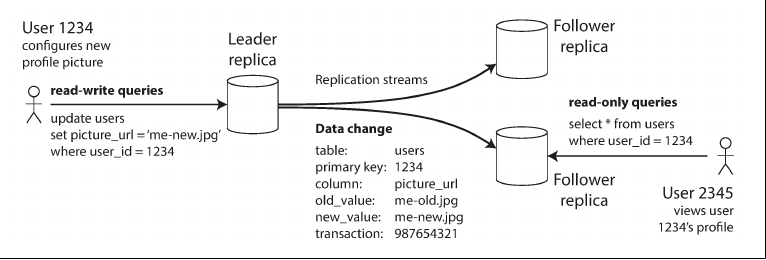
\includegraphics[width=70mm, height=30mm, scale=0.1]{img/replica/leader_replicatn.png}

    \column{0.4\textwidth}
    \begin{itemize}
      \item Also called master-slave replication
      \item Considering synchronous/asynchronous config in databases.
      \item Using synchronous configuration is bad
      \item Async configuration is widely used in production deployments.
    \end{itemize}
  \end{columns}
\end{frame}

% -------------------------------------

\begin{frame}{leader follower copying strategy}
  \centering{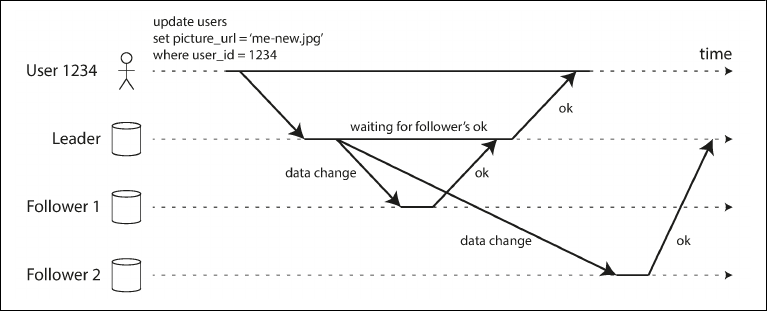
\includegraphics[width=70mm, height=30mm, scale=0.1]{img/replica/leader_replica_sync_async_follower.png}}
\end{frame}

% -------------------------------------

\begin{frame}{Follower setup without downtime}
  \begin{itemize}
      \pause
    \item Take a snapshot of the leader database at a specific time intervals
      \pause
    \item copy the snapshot to the new follower node.
      \pause
    \item followers connect to leaders \& retrieves data changes happened since the snapshot was taken
      \pause
    \item when followers has processed the backlog of data changes since the last snapshot was taken, it is in sync.
      \pause
  \end{itemize}
\end{frame}

% -------------------------------------

\begin{frame}{Handling node outage in Leader-based replication}
  How do you achieve high availability in this architecture ?
  \begin{itemize}
      \pause
    \item Follower failure: Catch-up recovery
      \pause
      \begin{itemize}
        \item Each follower maitains a backlog
      \end{itemize}
      \pause
    \item Leader failure
      \pause
      \begin{itemize}
      \item one of its followers takes the leader
      \item clients need to be reconfigured to send writes to new leader
      \item other followers need to start consuming data changes from new leader.
      \item old leader joins back as normal follower
      \end{itemize}
  \end{itemize}
\end{frame}

% -------------------------------------

\begin{frame}{Multi-leader based replication}
  \begin{columns}
    \column{0.6\textwidth}
    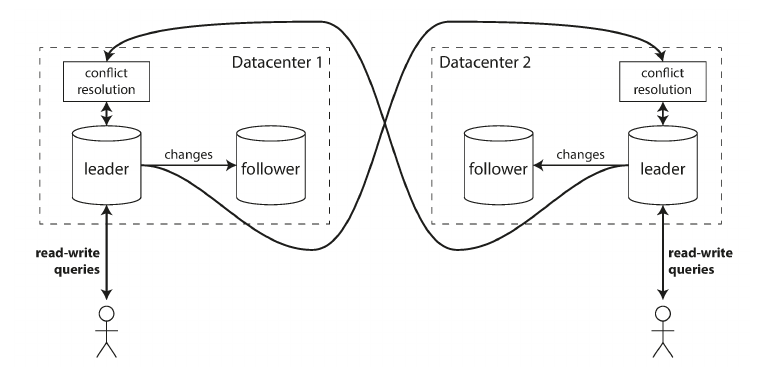
\includegraphics[width=70mm, height=30mm, scale=0.1]{img/replica/multi_leader_replication.png}

    \column{0.4\textwidth}
    \begin{itemize}
      \pause
      \item natural extension of leader-based replica, allows more than 1 node to accept writes
      \pause
      \item each leader simultaneously acts as follower to each leader
      \pause
      \item mostly used in multi-data center operations
    \end{itemize}
  \end{columns}
\end{frame}

% -------------------------------------

\begin{frame}{Conflict resolution problem}
  \begin{itemize}
    \pause
    \item all replicas must arrive at the same final value.
    \item avoid conflict all-together
      \pause
      \begin{itemize}
        \item all writes for a particular record go through the same leader.
      \end{itemize}
    \item In worst case, you have to deal with concurrent writes
      \pause
    \item There is some research on conflict resolving
      \begin{itemize}
        \item Conflict-free replicated data types
        \item Mergeable persistent data structures
        \item Operation transformation
      \end{itemize}
  \end{itemize}
\end{frame}

% -------------------------------------

\begin{frame}{Multi-leader topologies}
  \centering{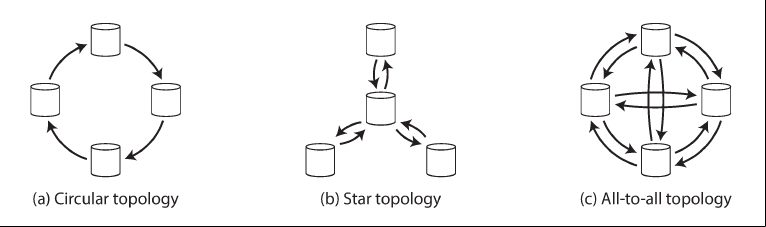
\includegraphics[width=80mm, height=30mm, scale=0.1]{img/replica/multi_leader_topology.png}}
\end{frame}

% -------------------------------------

\begin{frame}{Leaderless replication}
  \begin{columns}
    \column{0.6\textwidth}
    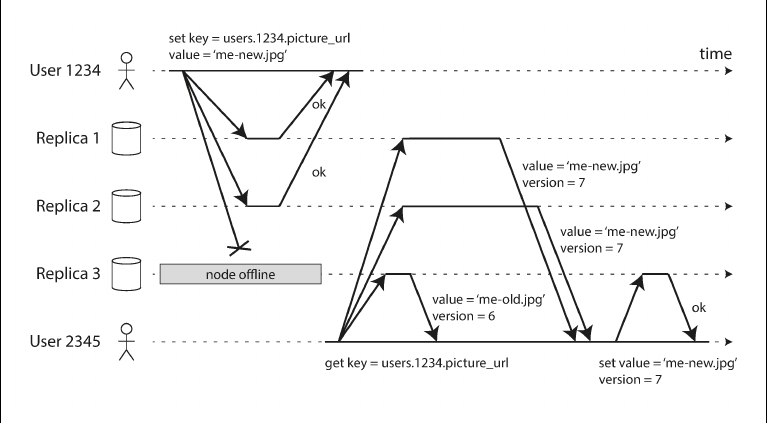
\includegraphics[width=70mm, height=30mm, scale=0.1]{img/replica/leader_less_replication_flow.png}

    \column{0.4\textwidth}
    \begin{itemize}
      \pause
      \item takes different approach instead of developing leader-follower concept
      \pause
      \item clients sends writes to replicas (can use broker to do this)
      \pause
      \item No restriction on ordering of writes
        \pause
      \item Amazon's DynamoDB is built using this concept
      \item examples include Cassandra, Riak 
    \end{itemize}
  \end{columns}
  

\end{frame}

% -------------------------------------

\begin{frame}{Leaderless write mechanisms}
  \begin{itemize}
    \item 3 replicas, 1 unavailable. how do you make up for unavailable replica ?
      \pause
    \item \textbf{Read Repair}
      \begin{itemize}
        \item version 6 value from replica 3, version 7 value from replica 1 \& 2 write version 7 to replica 3
      \end{itemize}
      \pause
    \item \textbf{Anti-entropy process}
      \begin{itemize}
        \item does reconcilation in background process
        \item writes are copied in unordered way
      \end{itemize}
  \end{itemize}
\end{frame}

% -------------------------------------

\begin{frame}{Quorums for reading and writing}
  Write processed on 2 out of 3 replicas. What if only 1 of 3 replicas accepted write ? How far can we push ?
  \begin{columns}
    \column{0.6\textwidth}
    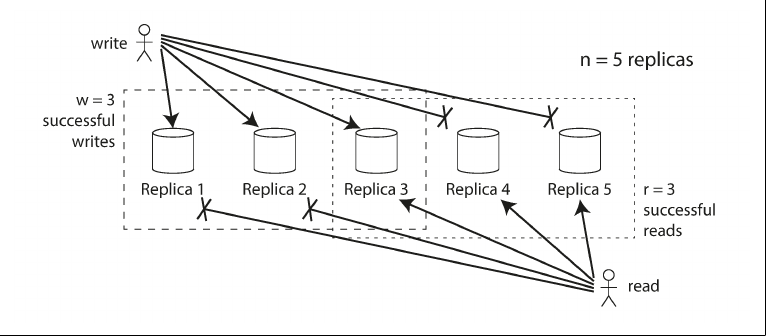
\includegraphics[width=70mm, height=30mm, scale=0.1]{img/replica/w_r_n.png}

    \column{0.4\textwidth}
    \pause
    \begin{corollary}
      $ w + r > n $
    \end{corollary}
    \pause
    \begin{itemize}
    \item If w $<$ n, we can still process writes if a node is missing
    \item If r $<$ n, we can still process reads if a node is missing
    \item n = 3, w = 2, r = 2, we can tolerate 1 unavailable node
    \item n = 5, w = 3, r = 3, we can tolerate 2 unavailable nodes
    \end{itemize}
  \end{columns}
\end{frame}

\subsection{Sharding/Partitions}
\begin{frame}{Sharding/Partitioning}
  Very large datasets, having high query throughput are broken down into partitions or shards.

  \pause
  \begin{columns}
    \column{0.4\textwidth}
    \begin{itemize}
    \item think of each partition as a small database of its own
    \item approaches for partitioning large datasets
      \begin{itemize}
        \item Partitioning by key range
        \item Partitioning by hash of a key
      \end{itemize}
    \end{itemize}
    
    \pause
    \column{0.6\textwidth}
    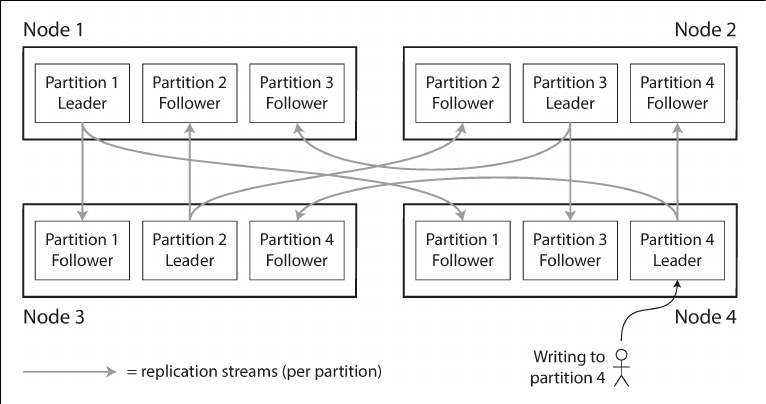
\includegraphics[width=55mm, height=25mm, scale=0.1]{img/shard_replica.png}
  \end{columns}
\end{frame}

% -------------------------------------

\section{Some strategies to scale up high-traffic web systems}
%\begin{frame}{Techniques to speed up data access}
%  Proven techniques employed that positively impacts speed factor of high traffic servers
%\end{frame}

% -------------------------------------

\subsection{Using Caches}
\begin{frame}{Using Caches}
  \begin{columns}
    \column{0.4\textwidth}
    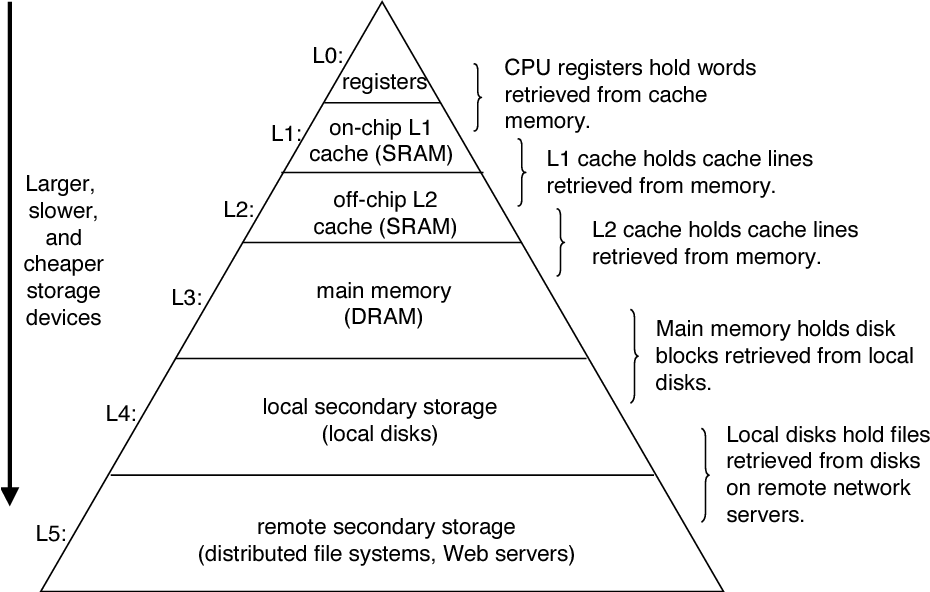
\includegraphics[width=50mm, height=25mm, scale=0.1]{img/mem_hierarchy.png}
    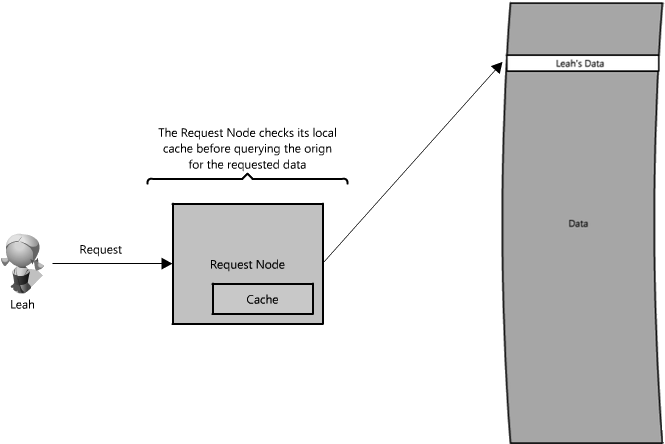
\includegraphics[width=50mm, height=25mm, scale=0.1]{img/simple_cache.png}
    \column{0.6\textwidth}
    \begin{itemize}
    \item any serious app will deploy a cache server
    \item usually placed in front of original data source
    \item algorithms like LRU(online algorithms) are widely used
    \item problem - If your system design uses load balancer, you will need to overcome high cache misses
    \end{itemize}
  \end{columns}
\end{frame}

% -------------------------------------

\begin{frame}{Overcoming cache misses}
  \begin{columns}
    \column{0.4\textwidth}
    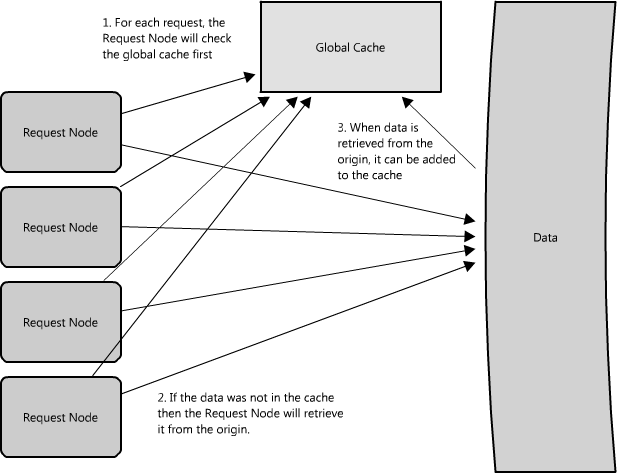
\includegraphics[width=50mm, height=25mm, scale=0.1]{img/global_cache2.png}
    \caption{figure 2}
    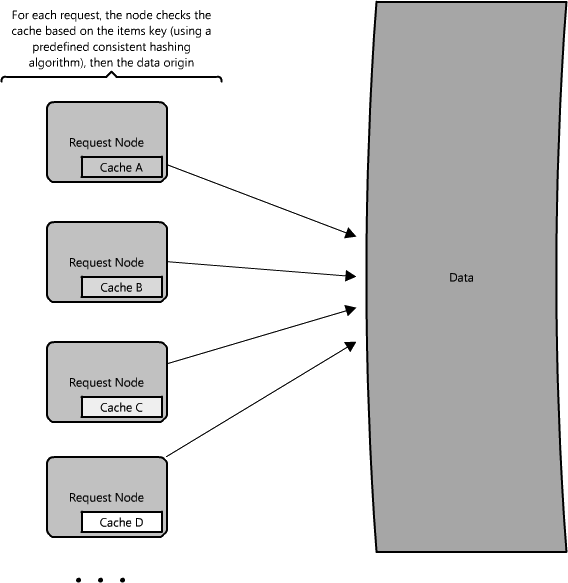
\includegraphics[width=50mm, height=25mm, scale=0.1]{img/dist_cache.png}
    \caption{figure 3}

    \column{0.6\textwidth}
    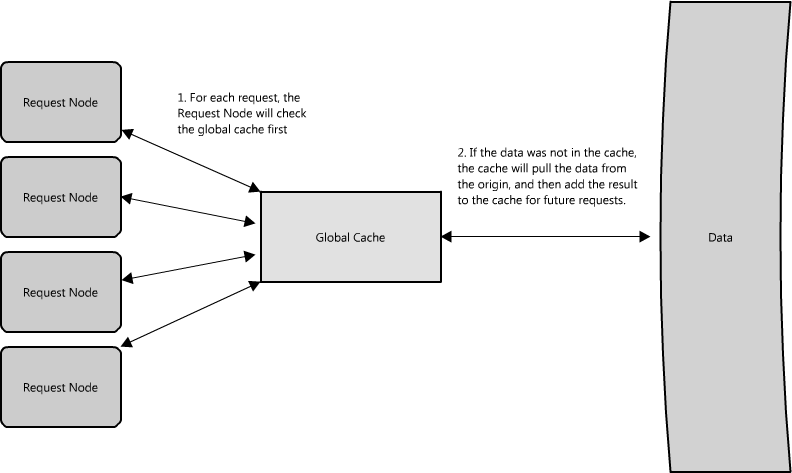
\includegraphics[width=50mm, height=25mm, scale=0.1]{img/global_cache.png}
    \caption{figure 1}
    \begin{description}
    \item[1st figure] handles eviction and data retrieval on its own
    \item[2nd figure] application handles eviction
    \item[3rd figure] each cache holds a portion of cached data
    \item[3rd figure] uses consistent hashing to lookup data across nodes
    \end{description}
  \end{columns}
\end{frame}


\subsection{Proxies}
\begin{frame}{Proxies}
 basic role is to receive requests from client and relay them to next node in line. 

 \pause
 \begin{columns}
    \column{0.4\textwidth}
    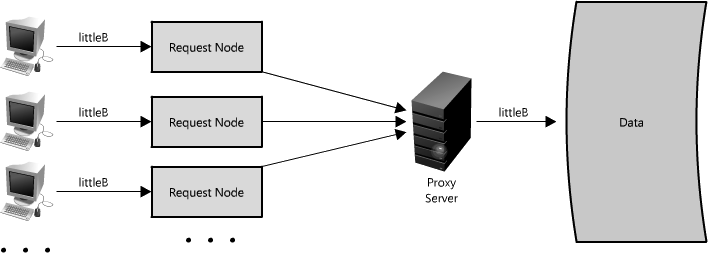
\includegraphics[width=55mm, height=25mm, scale=0.1]{img/proxy_collapse.png}
    \caption{figure 1}
    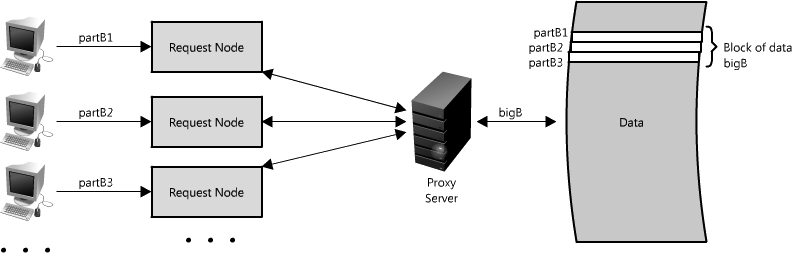
\includegraphics[width=55mm, height=25mm, scale=0.1]{img/proxy_collapse_spatial.png}
    \caption{figure 2}

    \column{0.6\textwidth}
    \begin{description}
    \item[1st figure] collapse similar requests into a single request
    \item[2nd figure] collapse requests for data that is spatially close together
    \end{description}
  \end{columns}
\end{frame}

% -------------------------------------

\subsection{Indexes}
\begin{frame}{Indexes}
  A very common, popular and important technique used to speedup data access

  \pause
 \begin{columns}
    \column{0.6\textwidth}
    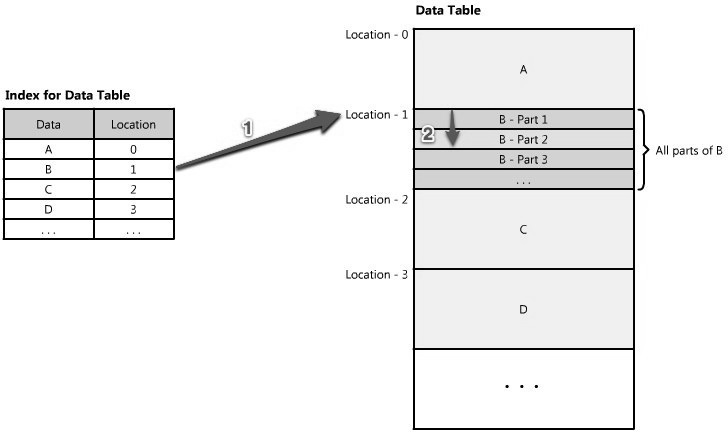
\includegraphics[width=60mm, height=30mm, scale=0.4]{img/indexing.jpg}
    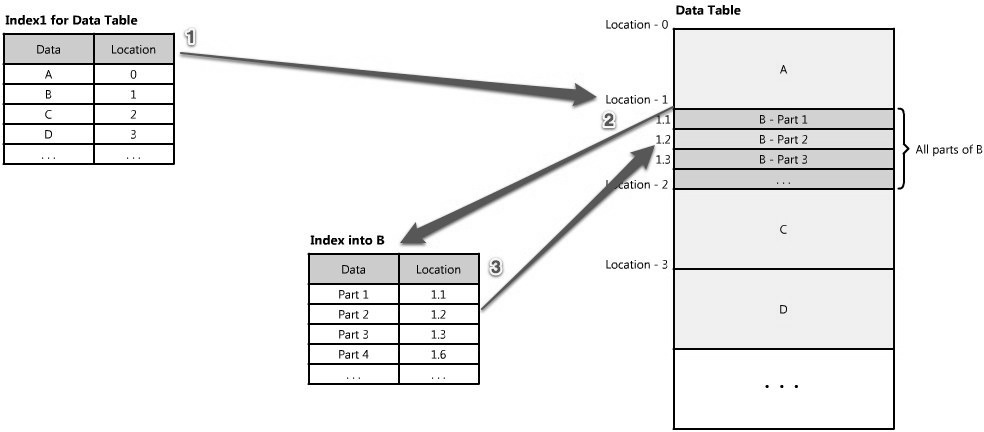
\includegraphics[width=60mm, height=30mm, scale=0.4]{img/indexlayers.jpg}

    \column{0.4\textwidth}
    \begin{itemize}
    \item the trick is to index your database based on users data access patterns
    \item In return for faster data access they do add write overhead and requiring updating indexes on each write
    \end{itemize}
  \end{columns}
\end{frame}

% -------------------------------------

\subsection{Load Balancers}
\begin{frame}{Load Balancers}
  Their role is to distribute incoming requests evenly, fairly among available servers. They serve as a
  brokers between client and logical nodes, handling lot of simultaneous connections.

  \pause
 \begin{columns}
    \column{0.6\textwidth}
    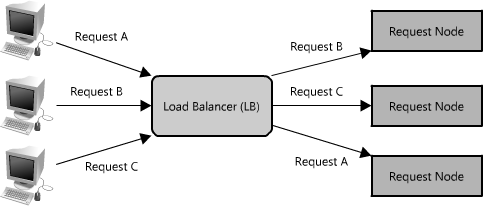
\includegraphics[width=60mm, height=30mm, scale=0.4]{img/loadBalancer.png}

    \column{0.4\textwidth}
    Algorithms used - 
    \begin{itemize}
    \item round robin
    \item just pick a random node
    \item selecting a node on a criteria - CPU, memory
    \end{itemize}
  \end{columns}
\end{frame}

% -------------------------------------

\subsection{Queues}
\begin{frame}{Queues}
  Queues solve a unique problem that load balancing, adding/removing servers cant solve.
  \pause
  \begin{columns}
    \column{0.6\textwidth}
    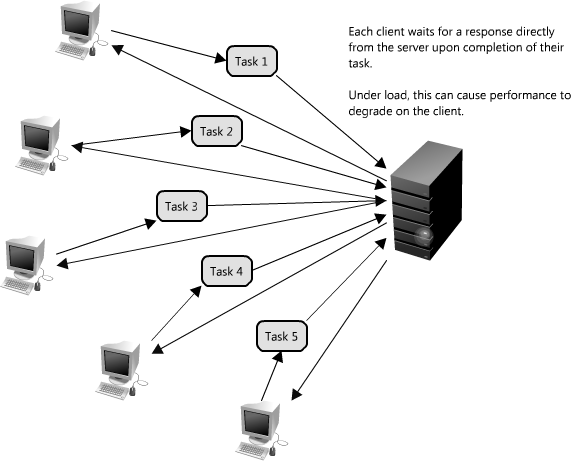
\includegraphics[width=55mm, height=30mm, scale=0.4]{img/queue_sync.png}
    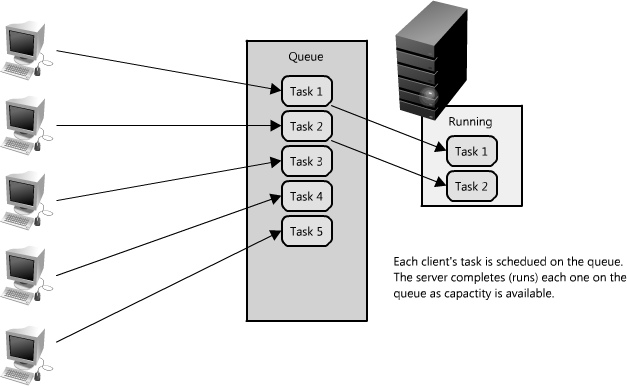
\includegraphics[width=55mm, height=30mm, scale=0.4]{img/queue_async.png}

    \column{0.4\textwidth}
    \begin{itemize}
    \item work in async manner
    \item client is given acknowledgement that request is served
    \item tasks range from as simple as write to a data store to as complex as extracting pdf from text
    \end{itemize}
  \end{columns}
\end{frame}

% -------------------------------------

\subsection{Naive Hashing}
\begin{frame}{Naive Hashing}
  \begin{columns}
    \column{0.5\textwidth}
    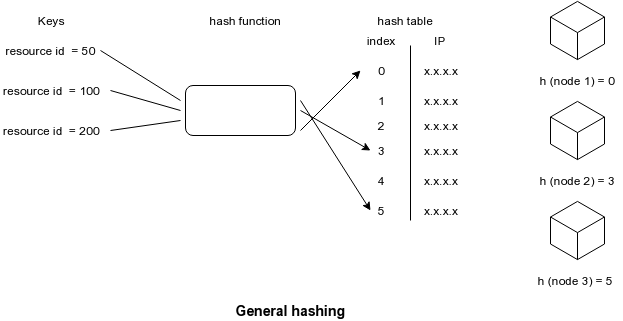
\includegraphics[width=60mm, height=30mm, scale=0.9]{img/naive hashing.png}

    \column{0.5\textwidth}
    some assumptions - 
    \begin{itemize}
    \item no. of nodes serving request never change
    \item repeated request can be served using cache
    \item requires rehashing every single key, caches get obselete.
    \end{itemize}
  \end{columns}
\end{frame}

% -------------------------------------

\subsection{Consistent Hashing}
\begin{frame}{Consistent Hashing}
  Incoming requests and serving nodes are placed onto a virtual ring structure called \textit{hashring}

  \centering{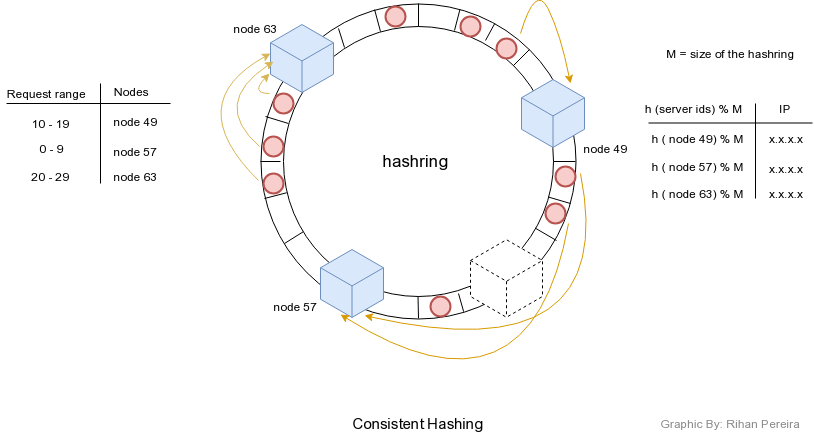
\includegraphics[width=75mm, height=40mm, scale=0.9]{img/consistent_hashing.png}}
    
  \begin{itemize}
    \item placement of server nodes is not fixed on the ring, instead are placed at random locations
    \item each server owns a range of hashring
    \item No worries on adding new servers or server disruptions
    \item only rehashing of affected portion of requests is required
  \end{itemize}
\end{frame}

\section{References}
\begin{frame}
  \bibliographystyle{unsrt}
  \begin{thebibliography}{99}
  \bibitem[Paper 1]{ref1} James Hamilton,  \newblock \emph{On Designing and Deploying Internet-Scale Services}, \textbf{2007}.
  \bibitem[Paper 2]{ref2} Twitter,  \newblock \emph{Automatic Management of Partitioned, Replicated Search Services}, \textbf{2011}.
  \bibitem[Paper 3]{ref3} http://blog.acolyer.org/, \newblock \emph{The morning Paper}.
  \bibitem[Paper 4]{ref3} http://aosabook.org, \newblock \emph{The architecture of open source applications}.
  \bibitem[Paper 5]{ref3} http://book.mixu.net/distsys, \newblock \emph{Distributed Systems: fun and profit}.
  \end{thebibliography}
\end{frame}

\section{Thats it}
\begin{frame}{}
  \centering{Thank you! Questions ?}
\end{frame}
\end{document}
%%% Local Variables:
%%% mode: latex
%%% TeX-master: t
%%% End:
